\documentclass[tikz, margin=5mm]{standalone}

\begin{document}

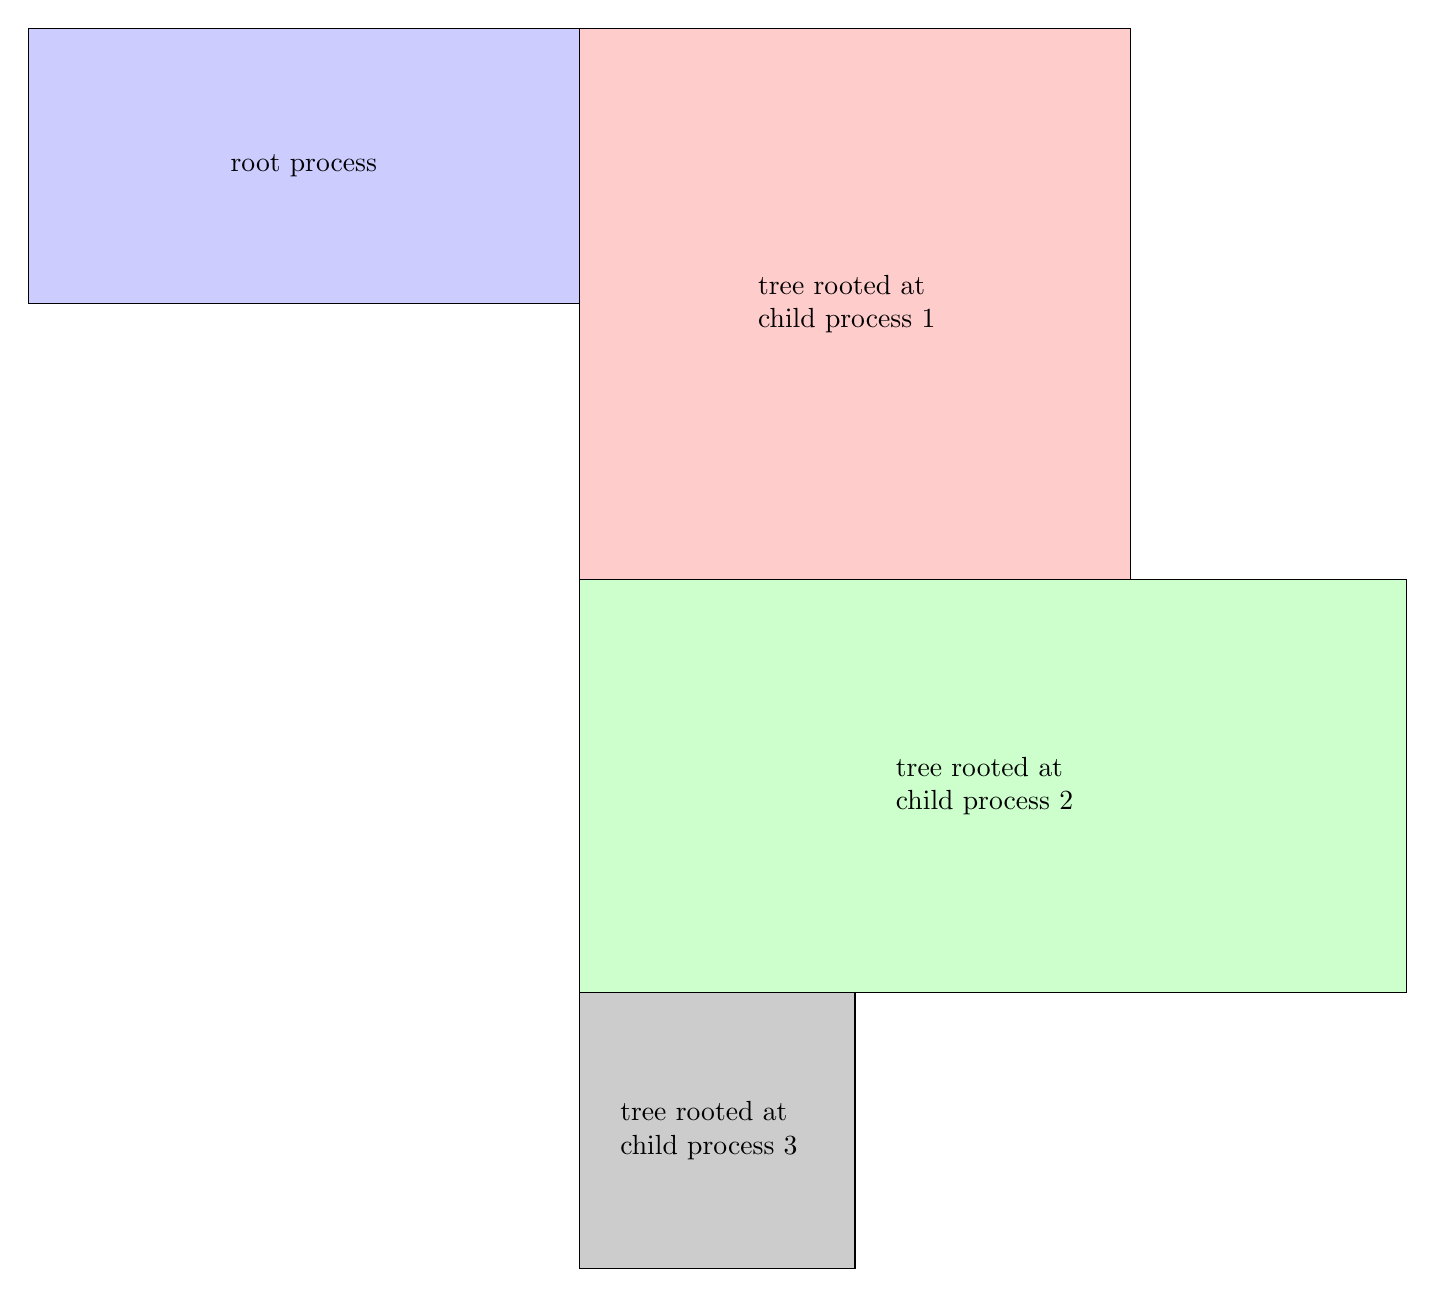
\begin{tikzpicture}
  \def\R{7}
  \draw [fill=blue!20!white] (0,0) rectangle (\R,-0.5*\R);
  \draw (0.5*\R,-0.25*\R) node {root process};
  \draw [fill=red!20!white] (\R,0) rectangle (2*\R,-\R);
  \draw [text width=10*\R](1.5*\R, -0.5*\R) node {tree rooted at child process 1};
  \draw [fill=green!20!white] (\R,-\R) rectangle (2.5*\R,-1.75*\R);
  \draw [text width=10*\R](1.75*\R, -1.375*\R) node {tree rooted at child process 2};
  \draw [fill=black!20!white] (\R,-1.75*\R) rectangle (1.5*\R,-2.25*\R);
  \draw [text width=10*\R](1.25*\R, -2*\R) node {tree rooted at child process 3};
  
\end{tikzpicture}
\end{document}